
\section{\rm{H}adron calorimeter}
The hadron calorimeter (HCAL) of the CMS experiment is used to measure the 
energy deposited
by hadrons (protons, pions, neutrons, kaons, etc). It is also useful
in estimating the missing transverse energy (as described in Section~\ref{s:secMET}) 
which is attributed to the neutrinos and unknown particles such as the dark 
matter. The HCAL is made of alternating layers of absorbers and plastic scintillators.
The absorber is made of brasses and steels whereas the scintillators are made
of Bicron-BC408 and Kuraray-SCSN81. When a particle passes through the 
absorber, it produces hadronic showers (a cascade of secondary particles). The 
secondary particles of the shower interact with the scintillating material
producing photons. The photons are converted into an electronic signal by hybrid
photodiodes (HPDs). The HCAL is made up of 36 barrel, 36 endcap wedges 
(weight of 1 wedge = 26 tonnes), 70000 tiles, and contains over 400 
optical decoder units which take light to the HPDs.
\begin{figure}
  \centering
  \subfigure[A prototype of HCAL barrel
  \label{subfig:cms_hcal1}]
  {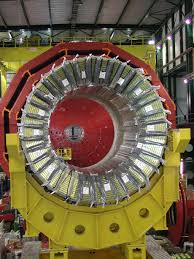
\includegraphics[width=0.31\linewidth]{Experiment/CMS/Image/HCAL/hcal1.jpg}}
  \hfil
  \subfigure[The actual HCAL endcap
  \label{subfig:sinti_hcal2}]
  {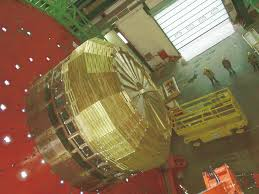
\includegraphics[width=0.55\linewidth]{Experiment/CMS/Image/HCAL/hcal2.jpg}}
	\caption{The CMS hadron calorimeter \cite{Collaboration_2008_CMS}. A prototype of 
	HCAL barrel is shown in silver color in (a). The actual endcap part of the HCAL 
	is shown in (b).}
  \label{fig:cms_hcal}
\end{figure}

Plastic (organic) scintillators are used in HCAL, unlike the inorganic scintillators 
of the ECAL. The organic scintillators have a wide range of varieties such as a
pure organic crystal (anthracene $\rm C_{14}\rm H_{10}$), organic liquids 
(p-terphenyl $\rm C_{18}\rm H_{14}$), and a plastic scintillator (polyethylene 
naphthalate). The typical gap between the electronic (vibrational) energy 
levels is 3-4\unit{eV} (0.15\unit{eV}). The scintillation mechanism in an organic scintillator
is shown in Figure~\ref{fig:cms_org_sinti}. At room temperature, all 
molecules having an energy about 0.025 eV are in the singlet ground state
($S_{00}$). When a particle passes through the scintillator, it transfers part of its 
kinetic energy to the molecules exciting them to higher states. The 
de-excitations from $S_2 \rightarrow S_1$ and $S_3 \rightarrow S_1$ are radiationless transitions.
That is, a photon is not produced in such a transition. However, as a result of 
these transitions, the population at $S_1$ increases considerably. The 
transitions from $S_1$ to lower energy states result in the emission of 
photons. There are two types of such transitions. The first is from 
$S_1 \rightarrow S_0$ called fluorescence, and the second is 
$S_1 \rightarrow T_1 \rightarrow S_0$ called phosphorescence. The light 
produced from such transitions is converted into electric signals by HPDs. 
The HPD uses photomultiplier-cum-semiconductor photodiode principle.  
\begin{figure}
  \begin{center}
  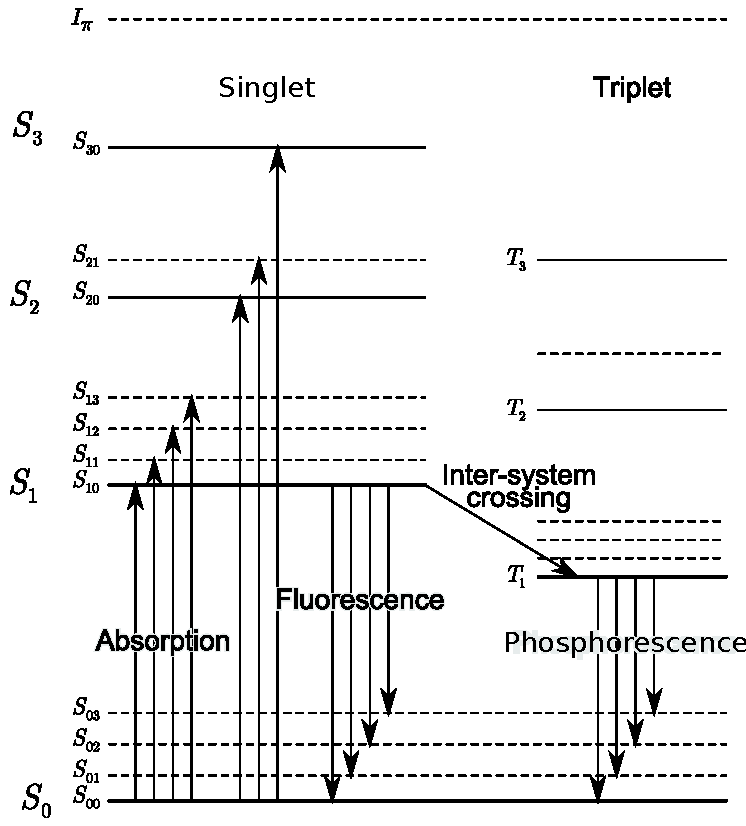
\includegraphics[width=0.5\linewidth]{Experiment/CMS/Image/HCAL/organic_sinti.pdf}
	\caption{The energy levels of a molecule of an organic scintillator 
	  \cite{wiki:orgSinti}. The ground state is $S_0$ followed by vibration
	  sublevels ($S_{01}, S_{02}$ etc). The $S_{1, 2, 3}$ are the excited 
	  singlet energy levels. In between the singlet, there are triplet energy 
	  levels shown as $T_{1, 2, 3}$. The fluorescence (phosphorescence) occurs
	  when there is a transition from $S_1 (T_1) \rightarrow S_{03, 02, 01, 00}$.}
  \label{fig:cms_org_sinti}
  \end{center}
\end{figure}


The HCAL calorimeters are placed in the barrel and endcap regions as shown in
Figure~\ref{fig:cms_hcal_pos} along with its various components. 
\begin{figure}
  \begin{center}
  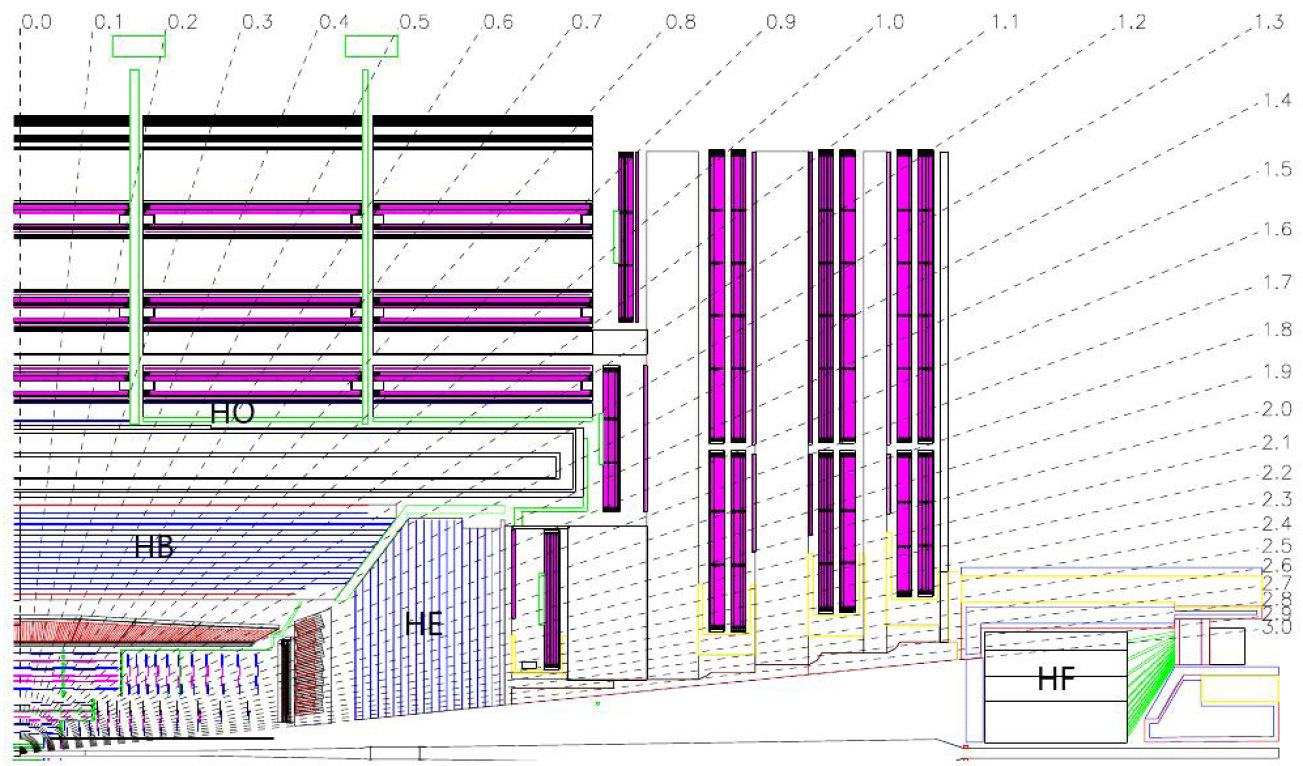
\includegraphics[width=0.75\linewidth]{Experiment/CMS/Image/HCAL/hcal.png}
	  \caption{The location of various components (HB, HO, HE, and HF) of 
	  the HCAL \cite{Isildak:2013kfa}.}
  \label{fig:cms_hcal_pos}
  \end{center}
\end{figure}
The hadron calorimeters are in the barrel (HB), endcap (HE), outer (HO), and 
forward (HF) region. The HO is placed outside of the magnetic solenoid acting
as a tail catcher. The HF is used to study jets in the forward region coming
from high radiations. More description of various components of the HCAL is given below:
\begin{itemize}[leftmargin=*]
  \item \textbf{Hadron Barrel}:
	The HB has a fine and uniform granularity in the $\eta-\phi$ plane, 
	for example, $\Delta\eta\times\Delta\phi = 0.087\times 0.087$.
	Due to high thickness, around 7-11 times of the interaction length,
	the HB stops almost all the hadrons passing through it.
  \item \textbf{Hadron Outer}:
	Even though all the hadrons are supposed to be stopped in the HB, there
	is a chance for high energetic hadrons to go outside the HB and magnetic
	solenoid. To measure the energy of hadronic showers from such hadrons,
	the HO is placed outside the magnet. The HO covers $|\eta| = 1.26$ range. 
  \item \textbf{Hadron Endcap}: The HE covers the $1.3\geq |\eta|\geq 3.0$
	region, with 14 additional calorimeter towers. Being close to the beam
	pipe, it is radiation hard. The response of the HE is regularly 
	calibrated during the data taking. The HB and HE overlap in the 
	1.305 $\geq |\eta| \geq 1.392$ region.
  \item \textbf{Hadron Forward}: The HF is located in the forward region
	in the range $1.3\geq |\eta| \geq 3.0$, and $z = \pm$ 11.2 m from the
	collision point. The length of the HF is 1.65 m, divided into 900 towers.
	The hadronization product of the beam remnants and jets with very high
	$\eta$ value are detected by the HF.
\end{itemize}

The energy resolution of the HCAL is given by
\begin{equation}
	\left(\frac{\sigma}{E}\right)^2 = \left(\frac{s}{\sqrt{E}}\right)^2 + c^2,
\end{equation}
where the energy of hadron ($E$) is measured in \GeV, the constant 
$s = (0.847)$\GeV$^{1/2}$ and $c = 0.074$ for all part of 
the HCAL except the HF. For the HF, $s = 1.98 $ \GeV $^{1/2}$ and $c = 0.09$.
The pion energy resolution from the HCAL is shown in Figure~\ref{fig:cms_hcal_reso}.
For low $E$, the resolution is poor, while for $E > 100$ \GeV, it lies in 5-10\%
range.
\begin{figure}
  \begin{center}
  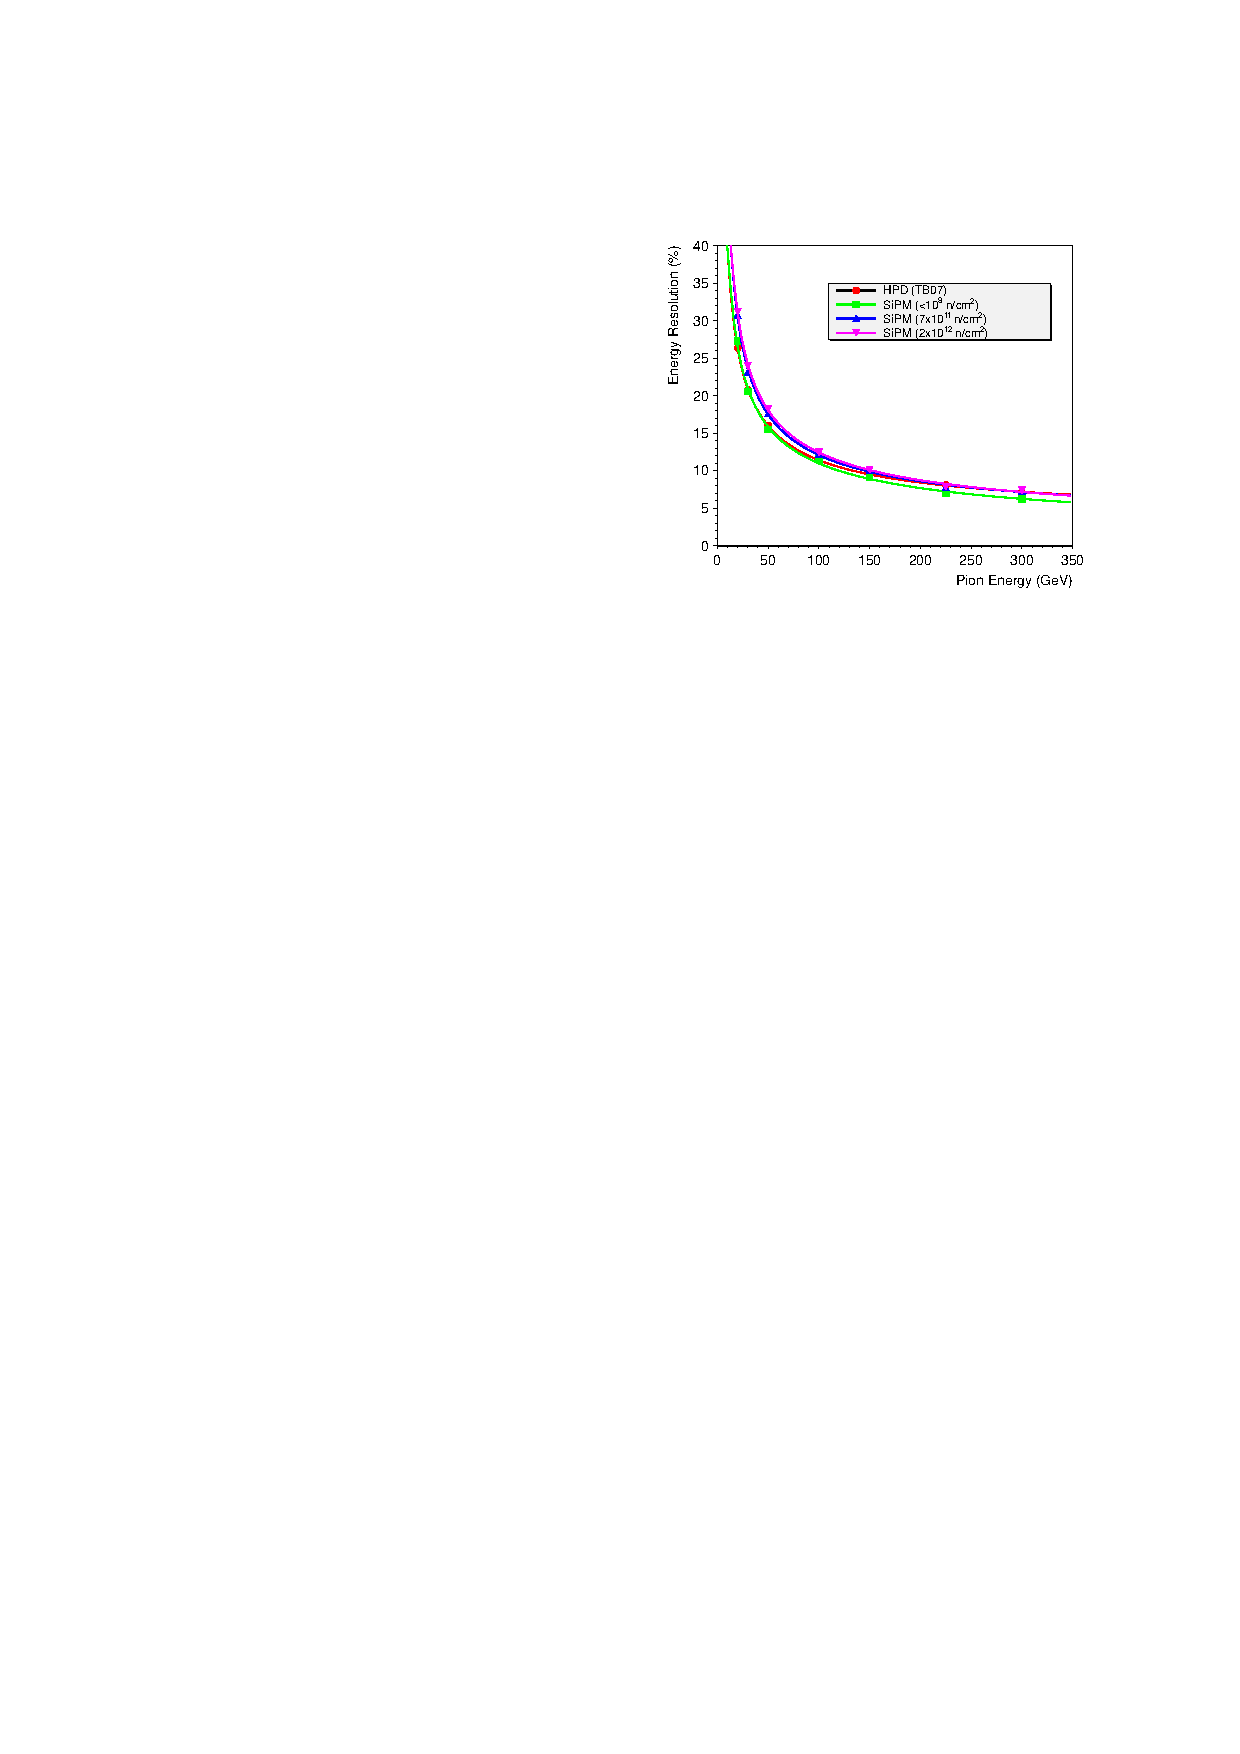
\includegraphics[width=0.50\linewidth]{Experiment/CMS/Image/HCAL/cms_hcal_reso.pdf}
  \caption{The HCAL energy resolution as a function of pion energy measured using
	  hybrid photodiodes, and silicon photomultipliers with different pixel
	  density \cite{Mans:1481837}.}
  \label{fig:cms_hcal_reso}
  \end{center}
\end{figure}
